\documentclass[11pt,a4paper]{article}
\usepackage[margin=2.4cm]{geometry}
\usepackage{fontspec}
\setmainfont{texgyretermes}[Extension=.otf,UprightFont=*-regular,BoldFont=*-bold,ItalicFont=*-italic,BoldItalicFont=*-bolditalic]
\setsansfont{texgyreheros}[Extension=.otf,UprightFont=*-regular,BoldFont=*-bold,ItalicFont=*-italic,BoldItalicFont=*-bolditalic]
\setmonofont{texgyrecursor}[Extension=.otf,UprightFont=*-regular,BoldFont=*-bold,ItalicFont=*-italic,BoldItalicFont=*-bolditalic,Scale=0.95]
\usepackage{graphicx}
\usepackage{booktabs}
\usepackage{tabularx}
\usepackage{xcolor}
\usepackage{listings}
\usepackage{enumitem}
\usepackage[hidelinks]{hyperref}
\usepackage{caption}
\captionsetup{font=small,labelfont=bf}
\graphicspath{{figures/}}
\definecolor{codebg}{gray}{0.95}
\lstset{basicstyle=\ttfamily\small,backgroundcolor=\color{codebg},frame=none,breaklines=true,
        columns=fullflexible,keepspaces=true,showstringspaces=false,xleftmargin=4pt,aboveskip=6pt,belowskip=6pt}
\setlist{itemsep=2pt,topsep=4pt}
\newcommand{\code}[1]{\texttt{#1}}

\title{\textbf{xbnh-gpu}\\[4pt]\large XBeach non-hydrostatic on the GPU: installation, use and validation}
\author{Stefano Biondi}
\date{Version 1.0, October 2026}

\begin{document}
\sloppy
\maketitle

\begin{abstract}
\noindent xbnh-gpu is a CUDA implementation of the one-layer non-hydrostatic (phase-resolving) flow solver
of XBeach (trunk revision 6167). It reads XBeach input decks unchanged and writes XBeach-format output.
Against Fortran XBeach it reproduces the significant wave height within 0.2\,\% and the mean current
within 0.6 to 0.8\,\% when compared with serial XBeach. With cyclic lateral boundaries it is as close to
XBeach MPI as XBeach MPI is to itself at a different number of ranks. On a full Estero Island storm deck
(8.7 million cells), one RTX~2000 Ada GPU ran 4.1 times (double precision) and 9.5 times (single
precision) faster than XBeach on 13 CPU cores. This guide explains how to install the code without
administrator rights, build it for any recent NVIDIA GPU, run existing XBeach decks, and verify the
results against a reference XBeach build that the repository also sets up.
\end{abstract}

\tableofcontents
\newpage

%=====================================================================================================
\section{What the code does}

XBeach in non-hydrostatic mode (\code{wavemodel = nonh}) resolves individual waves with a depth-averaged
momentum equation plus a vertical momentum equation and a non-hydrostatic pressure. The pressure is found
from a Poisson equation at every time step. These equations are local stencil operations on a structured
grid, which suit GPUs well: the cost is set by memory bandwidth, and a GPU has several times the bandwidth
of a CPU socket.

xbnh-gpu follows the XBeach Fortran source routine by routine, each routine becoming one or more CUDA
kernels:
\begin{itemize}
\item wet and dry cells and the time step (\code{wetcells.F90}, \code{timestep.F90});
\item boundary conditions, tide and wind (\code{boundaryconditions.F90}, \code{compute\_tide\_zs0.F90},
      \code{readwind.F90});
\item momentum, viscosity and friction (\code{flow\_timestep.F90}, \code{bedroughness.F90});
\item the non-hydrostatic predictor, breaking and pressure correction (\code{nonh.F90});
\item second-order advection (\code{flow\_secondorder.F90}).
\end{itemize}
Where the Fortran depends on its sequential loop order, the GPU code reproduces the same result. This
covers the neighbour checks of the breaking switch and two loop variables that XBeach reuses from earlier
loops when it sets the vertical velocity at points outside the pressure solve.

There are two intentional differences.
\begin{enumerate}
\item \textbf{Pressure solver.} XBeach uses SIP, an incomplete-LU sweep that is sequential by
construction. xbnh-gpu solves the same five-diagonal system with Jacobi-preconditioned BiCGStab to a
relative residual of $10^{-3}$ (key \code{gpu\_solver\_acc}). Agreement with XBeach stops improving below
this tolerance.
\item \textbf{Cyclic laterals.} XBeach supports \code{cyclic = 1} only under MPI, where the halo rows
1--2 and $n_y$--$n_y+1$ are copied from the opposite side of the domain (period $n_y-3$ rows). xbnh-gpu
keeps the whole domain in one block, makes the same halo copies after every update of a prognostic field,
and solves the pressure equation with periodic coupling. XBeach MPI does not exchange the velocities
between the pressure correction and the continuity equation (section~\ref{sec:numerics}); xbnh-gpu does.
\end{enumerate}

%=====================================================================================================
\section{Requirements}

\begin{itemize}
\item An NVIDIA GPU with compute capability 6.0 or newer: Pascal (P100, GTX 10xx) and later, including
      V100, T4, RTX 20xx/30xx/40xx, RTX Ada, A100 and H100. Check yours with \code{nvidia-smi
      --query-gpu=name,compute\_cap --format=csv}.
\item The NVIDIA driver, version 525.60 or newer (CUDA 12). On Windows, use WSL2 with the normal Windows
      NVIDIA driver; nothing GPU-related is installed inside WSL.
\item Linux x86-64, or Windows 10/11 with WSL2 (Ubuntu). Installing WSL itself may need administrator
      rights once; everything after that runs in user space.
\item About 3\,GB of disk for the build environment, and 2\,GB more for the optional reference XBeach.
\item GPU memory: about 0.8\,kB per grid cell in double precision and about half of that in single precision. An
      8.7-million-cell grid used 6.8\,GB in double precision.
\end{itemize}
No administrator rights are needed. The CUDA compiler, a compatible host C++ compiler, Python, and for
the reference model gfortran and Open MPI, all come from conda-forge through micromamba. They are
installed in the user's home directory.

%=====================================================================================================
\section{Installation}

\subsection{Automatic}
\begin{lstlisting}[language=bash]
git clone <repository URL> xbnh-gpu
cd xbnh-gpu
./install.sh                  # GPU code only
./install.sh --with-xbeach    # GPU code and the reference Fortran XBeach (10-20 min more)
source env.sh                 # in every new shell
bash tests/run_tests.sh
\end{lstlisting}
\code{install.sh} does the following.
\begin{enumerate}
\item It checks that \code{nvidia-smi} works and prints the GPU, its compute capability and the driver.
\item It installs micromamba in \code{\textasciitilde/.local/bin} if it is not already on the PATH.
      Environments go to \code{\$MAMBA\_ROOT\_PREFIX}, which defaults to \code{\textasciitilde/micromamba}.
\item It creates the environment \code{xbnh-gpu} from \code{environment.yml}: CUDA 12.6 \code{nvcc}, GCC
      13, make, Python 3.11 with NumPy, pandas and Matplotlib.
\item It builds \code{bin/xbnh\_gpu} (double precision) and \code{bin/xbnh\_gpu\_sp} (single precision)
      for the GPU in the machine (\code{ARCH=native}).
\item With \code{--with-xbeach}, it also creates \code{xbnh-xbeach} (gfortran 13, Open MPI, autotools,
      Subversion) and runs \code{xbeach/build\_xbeach.sh} (section~\ref{sec:xbeach}).
\item It writes \code{env.sh}, which activates the environment, puts \code{bin/} on the PATH, and sets
      \code{XBEACH\_SERIAL} and \code{XBEACH\_MPI} to the reference executables.
\end{enumerate}

\subsection{Manual}
With a CUDA toolkit (12.x) already available, for example on a cluster:
\begin{lstlisting}[language=bash]
module load cuda              # on HPC systems; any CUDA >= 11.8 with a C++20 host compiler
make ARCH=sm_80               # cross-compile, e.g. on a login node without a GPU
\end{lstlisting}
\begin{center}\small
\begin{tabular}{ll}
\toprule
\code{ARCH} & GPUs \\
\midrule
\code{native} & the GPU in this machine (default) \\
\code{sm\_60} & P100, GTX 10xx \\
\code{sm\_70} & V100 \\
\code{sm\_75} & T4, RTX 20xx \\
\code{sm\_80} & A100 \\
\code{sm\_86} & RTX 30xx, A40, A10 \\
\code{sm\_89} & RTX 40xx, RTX Ada, L4, L40 \\
\code{sm\_90} & H100 \\
\bottomrule
\end{tabular}
\end{center}

%=====================================================================================================
\section{Running a model}

xbnh-gpu runs in the folder that holds \code{params.txt}, like XBeach:
\begin{lstlisting}[language=bash]
cd my_deck
xbnh_gpu         # double precision
xbnh_gpu_sp      # single precision
\end{lstlisting}
\textbf{Use a separate folder from any XBeach run of the same deck.} The output files have XBeach names
and are overwritten. Linking the large input files avoids copies:
\begin{lstlisting}[language=bash]
mkdir run_gpu && cd run_gpu && cp ../xbeach_run/params.txt .
for f in z.grd nhbcflist.bcf nh_series00001.bcf water_elev.dat wind.txt hotstart_*; do
  ln -s ../xbeach_run/$f .; done
xbnh_gpu > stdout.txt
\end{lstlisting}

\subsection{Chaining segments}\label{sec:chain}
Long storms are usually run as a chain of shorter segments, each started from the state at the end of the
previous one. With \code{writehotstart = 1} the GPU code writes the nine files that \code{hotstart = 1}
reads (\code{hotstart\_zs, zb, uu, vv, wb, ws, breaking, umean, vmean} plus a six-digit number) every
\code{tinth} seconds, numbered from 1, in the same ASCII format as XBeach, so the files are interchangeable
between the two codes. A 900\,s segment written at its end is restarted with:
\begin{lstlisting}[language=bash]
mkdir seg2 && cd seg2
cp ../seg1/hotstart_*000001.dat .        # copy, do not link: seg2 writes files of the same names
cp ../deck_seg2/params.txt ../deck_seg2/water_elev.dat ../deck_seg2/wind.txt .
python $XBNH/tools/set_params.py params.txt hotstart=1 hotstartfileno=1 writehotstart=1 tinth=900 tstop=900
xbnh_gpu_sp > stdout.txt
\end{lstlisting}
Copy the hotstart files rather than linking them: a run that writes hotstart files of the same name would
write through the links into the previous segment. Time restarts from zero in every segment, as in XBeach,
so the tide, wind and boundary files of each segment start at its own $t = 0$.

\textbf{Spectral wave boundaries.} The GPU code reads a ready nonhydrostatic boundary series
(\code{wbctype = reuse} or \code{ts\_nonh}) but does not synthesise one from a spectrum. For a deck with
\code{wbctype = swan}, \code{jonstable} or similar, run the reference XBeach on it once with a short
\code{tstop} (a few seconds). XBeach writes \code{nhbcflist.bcf} and \code{nh\_series00001.bcf} for the
whole boundary duration before it starts stepping. Then set \code{wbctype = reuse} for the GPU run. Only the
offshore boundary matters for this step, so a copy of the deck cut to \code{nx = 4} with the same \code{ny},
\code{dy} and spectra gives the same series much faster. The synthesis runs on one core; on the Estero deck (5740 boundary rows, 900\,s) it takes one to two hours.

\subsection{Output}
\begin{itemize}
\item Global output for each variable listed under \code{nglobalvar} (\code{zs, u, v, uu, vv, ws, wb, hh,
      pres, breaking, zb, nuh, zs0}): one file \code{<var>.dat}, one float64 record of $(n_x+1)(n_y+1)$
      values per \code{tintg}, with $i$ (cross-shore) varying fastest. This is the XBeach
      \code{outputformat = fortran} layout. Read it in Python with
      \code{np.fromfile('zs.dat','<f8').reshape(-1, ny+1, nx+1)}.
\item Point output for each point under \code{npoints}: \code{<name>.dat}, one record per \code{tintp} of
      \code{[t, var1, var2, ...]} in float64. Points snap to the nearest cell centre, as in XBeach.
\item \code{xbgpu\_log.txt}: precision, number of steps, wall time, solver time and iterations, and cost per
      cell and step. Progress goes to standard output every 2000 steps.
\end{itemize}

\subsection{Single or double precision}
Single precision is about 2.3 times faster and uses about half the memory. In every test so far it gave
the same statistics as double precision. On the Estero deck it differed from double precision by 0.5\,\%
in $H_s$ and 0.001\,m/s in mean current. Consumer GPUs are much slower in double precision than in
single; data-centre GPUs (A100, H100) are not.

\subsection{GPU-specific keys}
\begin{center}\small
\begin{tabularx}{\textwidth}{llX}
\toprule
Key & Default & Meaning \\
\midrule
\code{gpu\_solver\_acc} & 0.001 & relative residual of the BiCGStab pressure solve \\
\code{gpu\_maxit} & 200 & maximum BiCGStab iterations per step (about 13 are typical) \\
\code{gpu\_hotstart\_keepuv} & 1 & keep \code{uu, vv} from the hotstart files. Trunk XBeach zeroes them after reading; 0 reproduces that. The reference build here keeps them (section~\ref{sec:xbeach}). \\
\bottomrule
\end{tabularx}
\end{center}
XBeach ignores these keys, apart from a warning about unknown parameters.

\subsection{Supported XBeach options}
\begin{center}\small
\begin{tabularx}{\textwidth}{lX}
\toprule
Group & Supported \\
\midrule
Model & \code{wavemodel = nonh}, \code{nonhq3d = 0}, \code{nhbreaker = 1}, \code{secorder = 1}, Smagorinsky (\code{smag}), Manning (\code{bedfriction = manning}) \\
Grid & uniform rectilinear, \code{vardx = 0}, \code{alfa = 0}, $n_y > 4$ \\
Offshore & \code{front = nonh\_1d}, \code{ARC = 1}; \code{wbctype = ts\_nonh} (\code{boun\_U.bcf}) or \code{reuse} (\code{nhbcflist.bcf}, one entry, scalar or vector file with U, V, Z) \\
Back & \code{back = wall}, \code{abs\_1d}, \code{abs\_2d} \\
Laterals & \code{left}, \code{right} = \code{neumann} or \code{wall}; or \code{cyclic = 1} \\
Water level & \code{zs0}, or \code{zs0file} with \code{tideloc = 1}; \code{tidetype = velocity} \\
Wind & \code{windv}, \code{windth}, or \code{windfile} \\
Restart & read: \code{hotstart = 1}, \code{hotstartfileno}; write: \code{writehotstart = 1} every \code{tinth} (XBeach ASCII format, files numbered from 1) \\
Output & \code{nglobalvar}, \code{npoints}, \code{tintg}, \code{tintp} (fortran format) \\
\bottomrule
\end{tabularx}
\end{center}
Not supported: two-layer \code{nonhq3d}, variable or rotated grids, sediment and morphology,
\code{tideloc} 2 or 4, several \code{nhbcflist} entries, netCDF output, and more than one GPU. Unsupported
options stop the program with a message instead of being ignored.

%=====================================================================================================
\section{Reference XBeach and tests}\label{sec:xbeach}

\code{xbeach/build\_xbeach.sh} downloads XBeach trunk r6167 from the Deltares Subversion server
(anonymous access) and applies two small patches (\code{xbeach/patch\_xbeach.py}). It then builds
\code{xbeach/dist\_serial/bin/xbeach} and \code{xbeach/dist\_mpi/bin/xbeach} (Open MPI), with Fortran
output only. The two patches are:
\begin{enumerate}
\item \textbf{Hotstart velocities} (\code{initialize.F90}). Trunk reads \code{uu, vv} from the hotstart
      files and then sets them to zero in \code{flow\_init}, so every restart starts from rest. The patch
      keeps them. The Estero runs used this build.
\item \textbf{Point output} (\code{postprocess.F90}). A missing comma in a log-message format makes runs
      with output points stop at start-up with ``Missing comma between descriptors''. This happens always
      in the serial build and intermittently under MPI. Only the message format changes.
\end{enumerate}
\code{cyclic = 1} needs the MPI build with at least two ranks: \code{mpirun -np 4 \$XBEACH\_MPI}.

\code{tests/run\_tests.sh} runs two small decks on the GPU in both precisions:
\begin{itemize}
\item a rip-channel beach (39\,k cells, 120\,s);
\item the Estero-feature deck (40\,k cells, 100\,s; cyclic laterals, \code{abs\_2d}, vector boundary,
      tide and wind files, point output);
\item a hotstart round trip on the Estero-feature deck: a 40\,s run writes a hotstart, a second run
      restarts from it, and the restarted water level and velocities must match to $10^{-6}$.
\end{itemize}
When the reference XBeach exists, the same decks run in Fortran XBeach and the agreement is checked
against thresholds. Otherwise the GPU statistics are checked against values stored in
\code{tests/reference.json}. The thresholds are several times the differences that XBeach itself shows
between rank counts.
The tests take two to five minutes. A passing run with the reference XBeach ends like this (the numbers
are from the RTX~2000 Ada):
\begin{lstlisting}
 Fortran XBeach (serial) against GPU
   Hs_rel          0.0014  (limit 0.01)  ok
   current_rel     0.0045  (limit 0.03)  ok
   zs_rms_m        0.0027  (limit 0.01)  ok
 ...
 Fortran XBeach (MPI, 2 ranks) against GPU
   Hs_rel          0.0032  (limit 0.02)  ok
   current_rel     0.0046  (limit 0.1)  ok
   zs_rms_m        0.0029  (limit 0.02)  ok
== 3. hotstart write and restart (Estero-feature deck)
 ...
   zs  max difference after restart 5.0e-09  (limit 1e-06)  ok
   uu  max difference after restart 5.0e-09  (limit 1e-06)  ok
   vv  max difference after restart 5.0e-09  (limit 1e-06)  ok
   PASS
tests passed: 9, failed: 0
\end{lstlisting}

%=====================================================================================================
\section{Validation}

\subsection{Rip-channel beach}
The deck has 39\,k cells and dx = 2\,m (\code{examples/rip\_beach}):
\begin{itemize}
\item a 1:50 slope with a shore-parallel bar cut by rip channels;
\item JONSWAP waves ($H_{m0}$ = 1\,m, $T_p$ = 8\,s) driven through \code{boun\_U.bcf}, for 200\,s.
\end{itemize}
Statistics are for $t \geq 60$\,s (Table~\ref{tab:rip}, Figure~\ref{fig:rip}).

\begin{table}[h]\centering\small
\caption{Rip-channel beach: differences against serial Fortran XBeach.}\label{tab:rip}
\begin{tabular}{lccc}
\toprule
Metric & GPU fp64 & GPU fp32 & XBeach MPI-4 \\
\midrule
$H_s$ map, relative RMSE & 0.16\,\% & 0.18\,\% & 0.36\,\% \\
Mean current, relative RMSE & 0.62\,\% & 0.61\,\% & 1.59\,\% \\
Set-up RMSE & 0.21\,mm & 0.21\,mm & 0.43\,mm \\
Instantaneous $z_s$, RMS difference & 3.5\,mm & 3.6\,mm & 4.1\,mm \\
\bottomrule
\end{tabular}
\end{table}

\begin{figure}[h]\centering
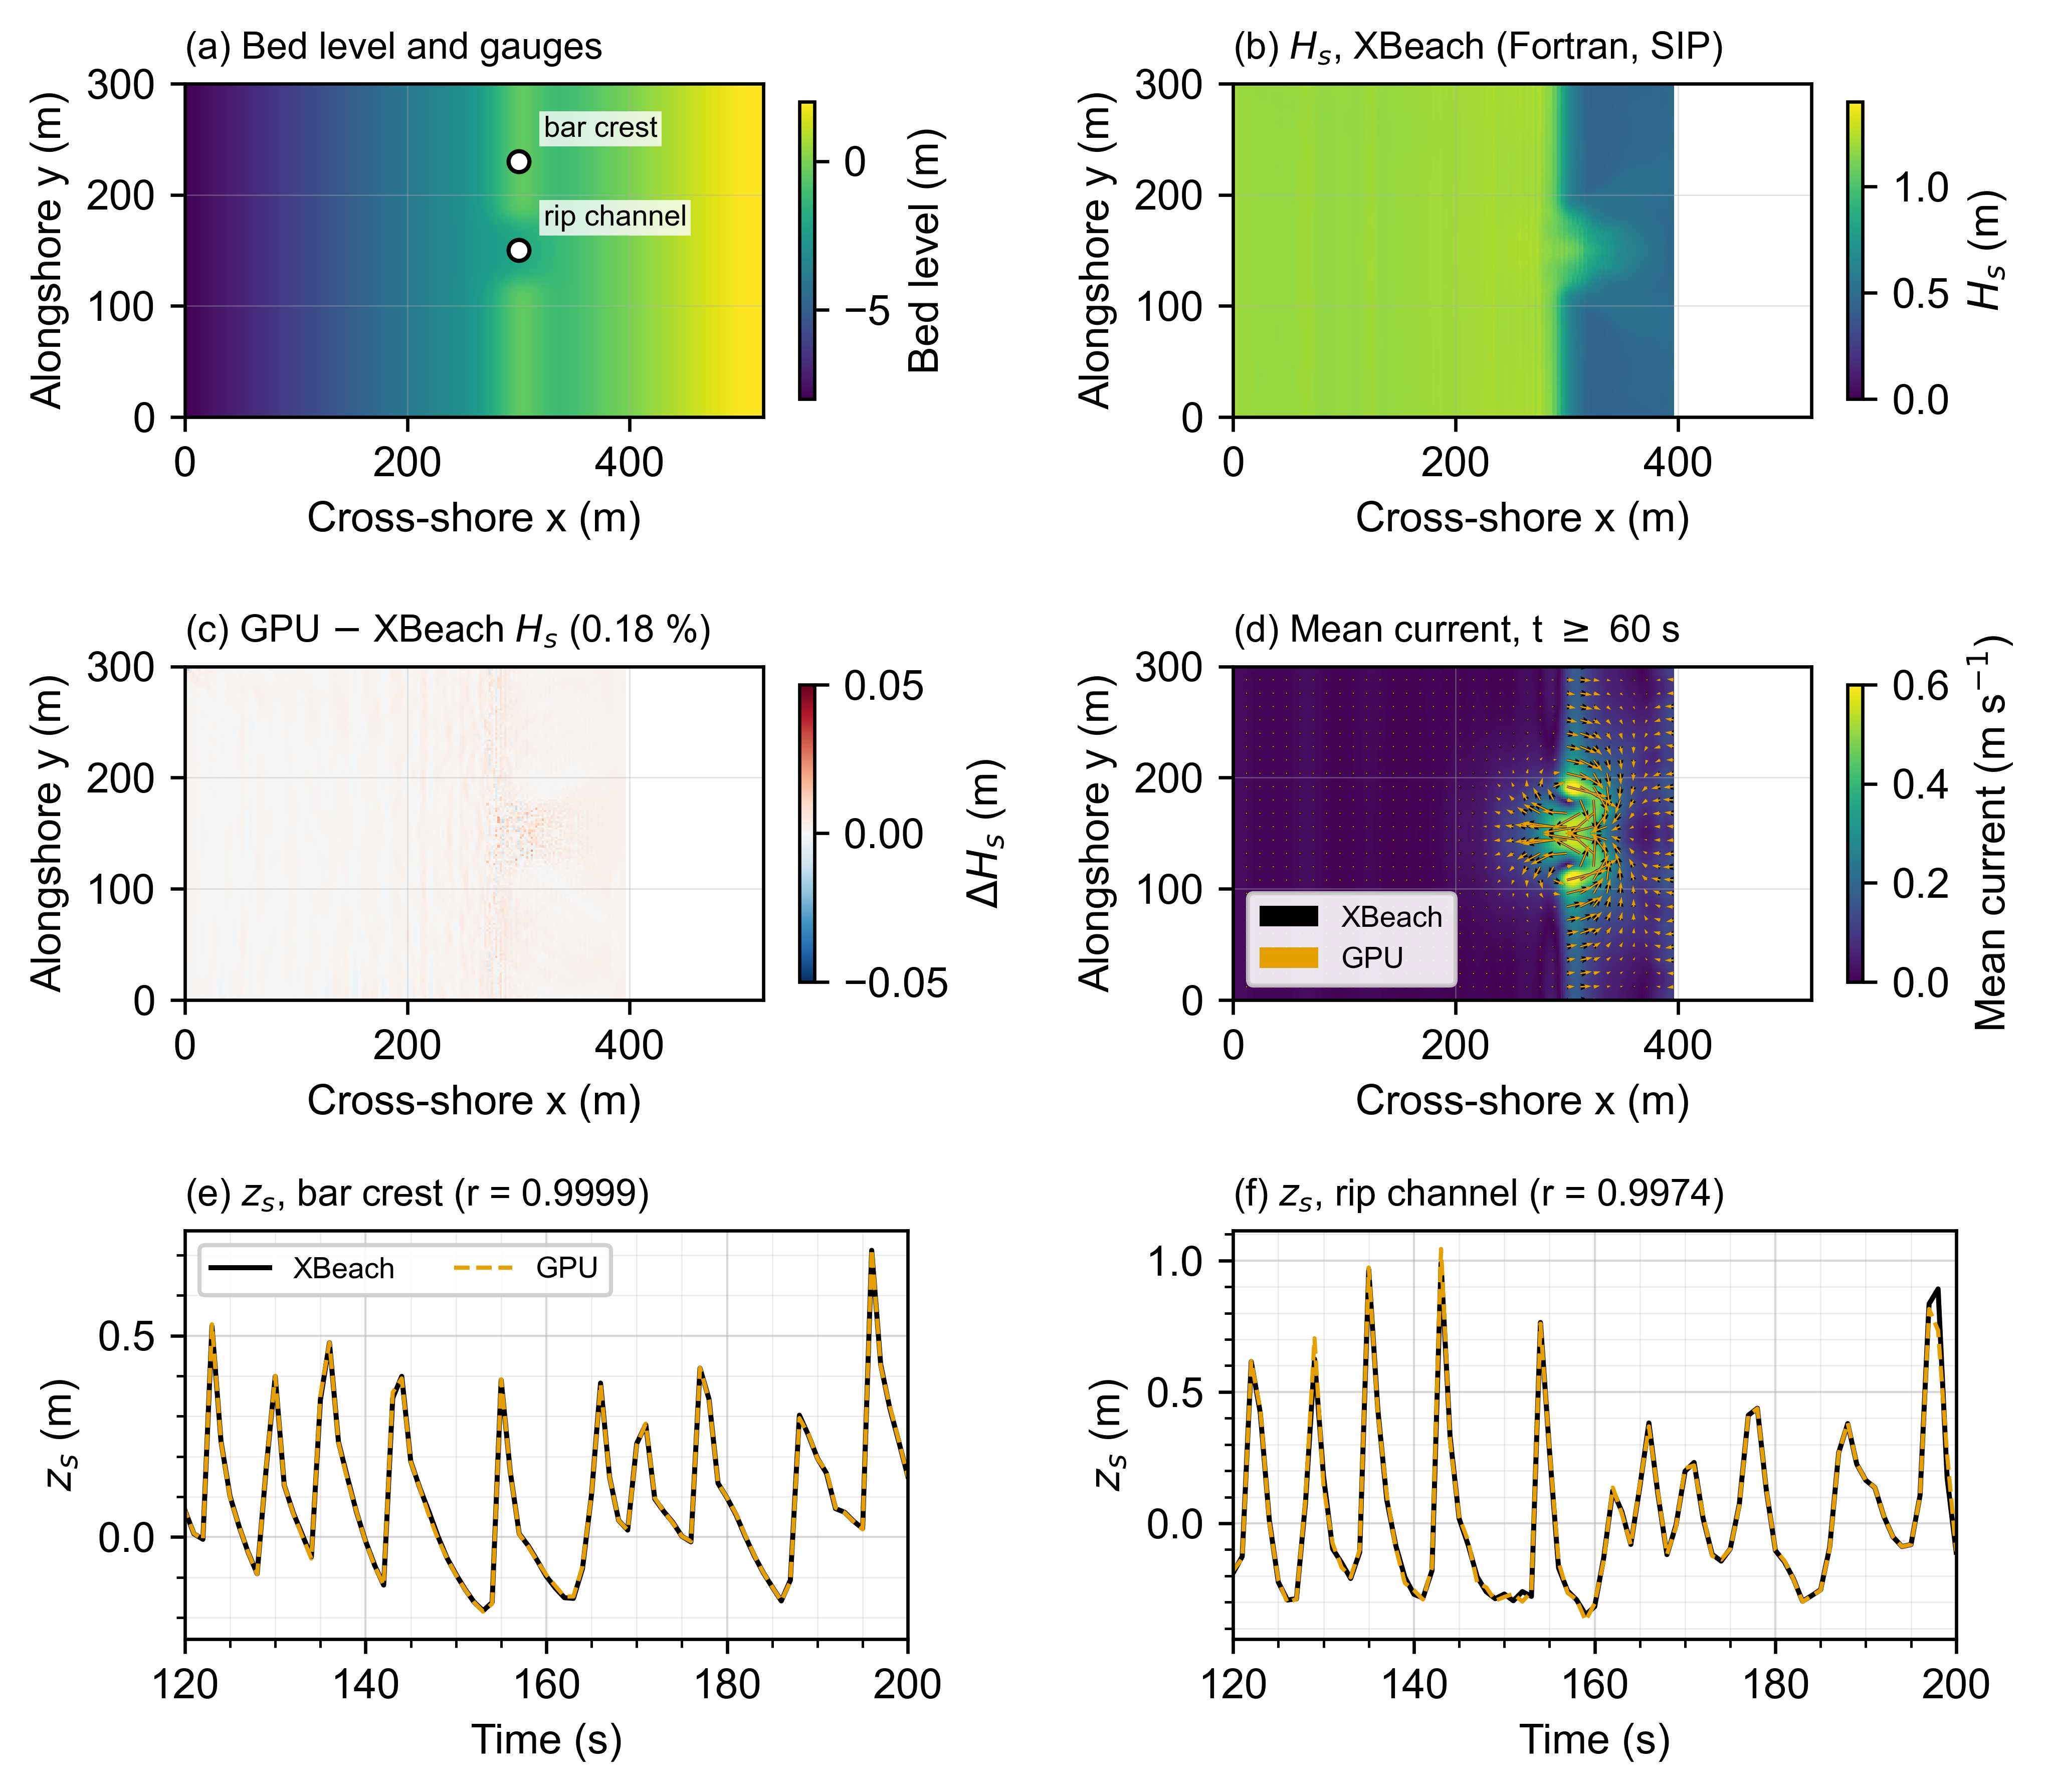
\includegraphics[width=0.82\textwidth]{validation_xbeach_vs_gpu.png}
\caption{Rip-channel beach. (a) Bed and gauges; (b) XBeach $H_s$; (c) GPU minus XBeach $H_s$; (d) mean
currents of both codes; (e, f) water level at the bar crest and in the rip channel.}\label{fig:rip}
\end{figure}

\subsection{Estero-feature deck}
\code{examples/estero\_features} combines every option of the Estero Island deck on 40\,k cells:
\begin{itemize}
\item cyclic laterals;
\item a wet \code{abs\_2d} back boundary;
\item a short-crested sea, 20$^\circ$ oblique, given as a vector U, V, Z file;
\item a rising tide from \code{zs0file} and a time-varying wind;
\item point output, and a hotstart written at 100\,s.
\end{itemize}
Table~\ref{tab:feat} lists the results.

\begin{table}[h]\centering\small
\caption{Estero-feature deck (relative RMSE of maps; $z_s$ as RMS difference).}\label{tab:feat}
\begin{tabular}{lcccc}
\toprule
Comparison & $H_s$ & Mean current & Longshore current & $z_s$ \\
\midrule
Serial XBeach vs GPU, hotstart, Neumann laterals & 0.20\,\% & 0.82\,\% & 1.2\,\% & 2.6\,mm \\
XBeach MPI-2 vs GPU, cyclic & 0.34\,\% & 2.0\,\% & 2.3\,\% & 4.7\,mm \\
XBeach MPI-4 vs GPU, cyclic & 0.54\,\% & 3.4\,\% & 4.9\,\% & 6.2\,mm \\
XBeach MPI-4 vs MPI-2 (yardstick) & 0.44\,\% & 2.8\,\% & 2.9\,\% & 5.5\,mm \\
\bottomrule
\end{tabular}
\end{table}

\subsection{Estero Island storm deck}
The full Estero Island deck (Hurricane Ian, 1515 $\times$ 5739 cells at 2\,m) was run for 300\,s from a
hotstart, with the same input files as XBeach on 13 MPI ranks. At the 50 output points the median
differences against XBeach were as follows:
\begin{itemize}
\item $H_s$: 1.9\,\%;
\item mean current: 0.002\,m/s, of a median 1.04\,m/s;
\item maximum speed: 0.8\,\%.
\end{itemize}
For scale, the same CPU run with only the wind drag changed differed by 3.4\,\%, 0.19\,m/s and 7.9\,\%
(Figure~\ref{fig:estero}). Wave phases at individual points begin to separate after about 230\,s, as they
do between any two XBeach runs with different rank counts.

\begin{figure}[h]\centering
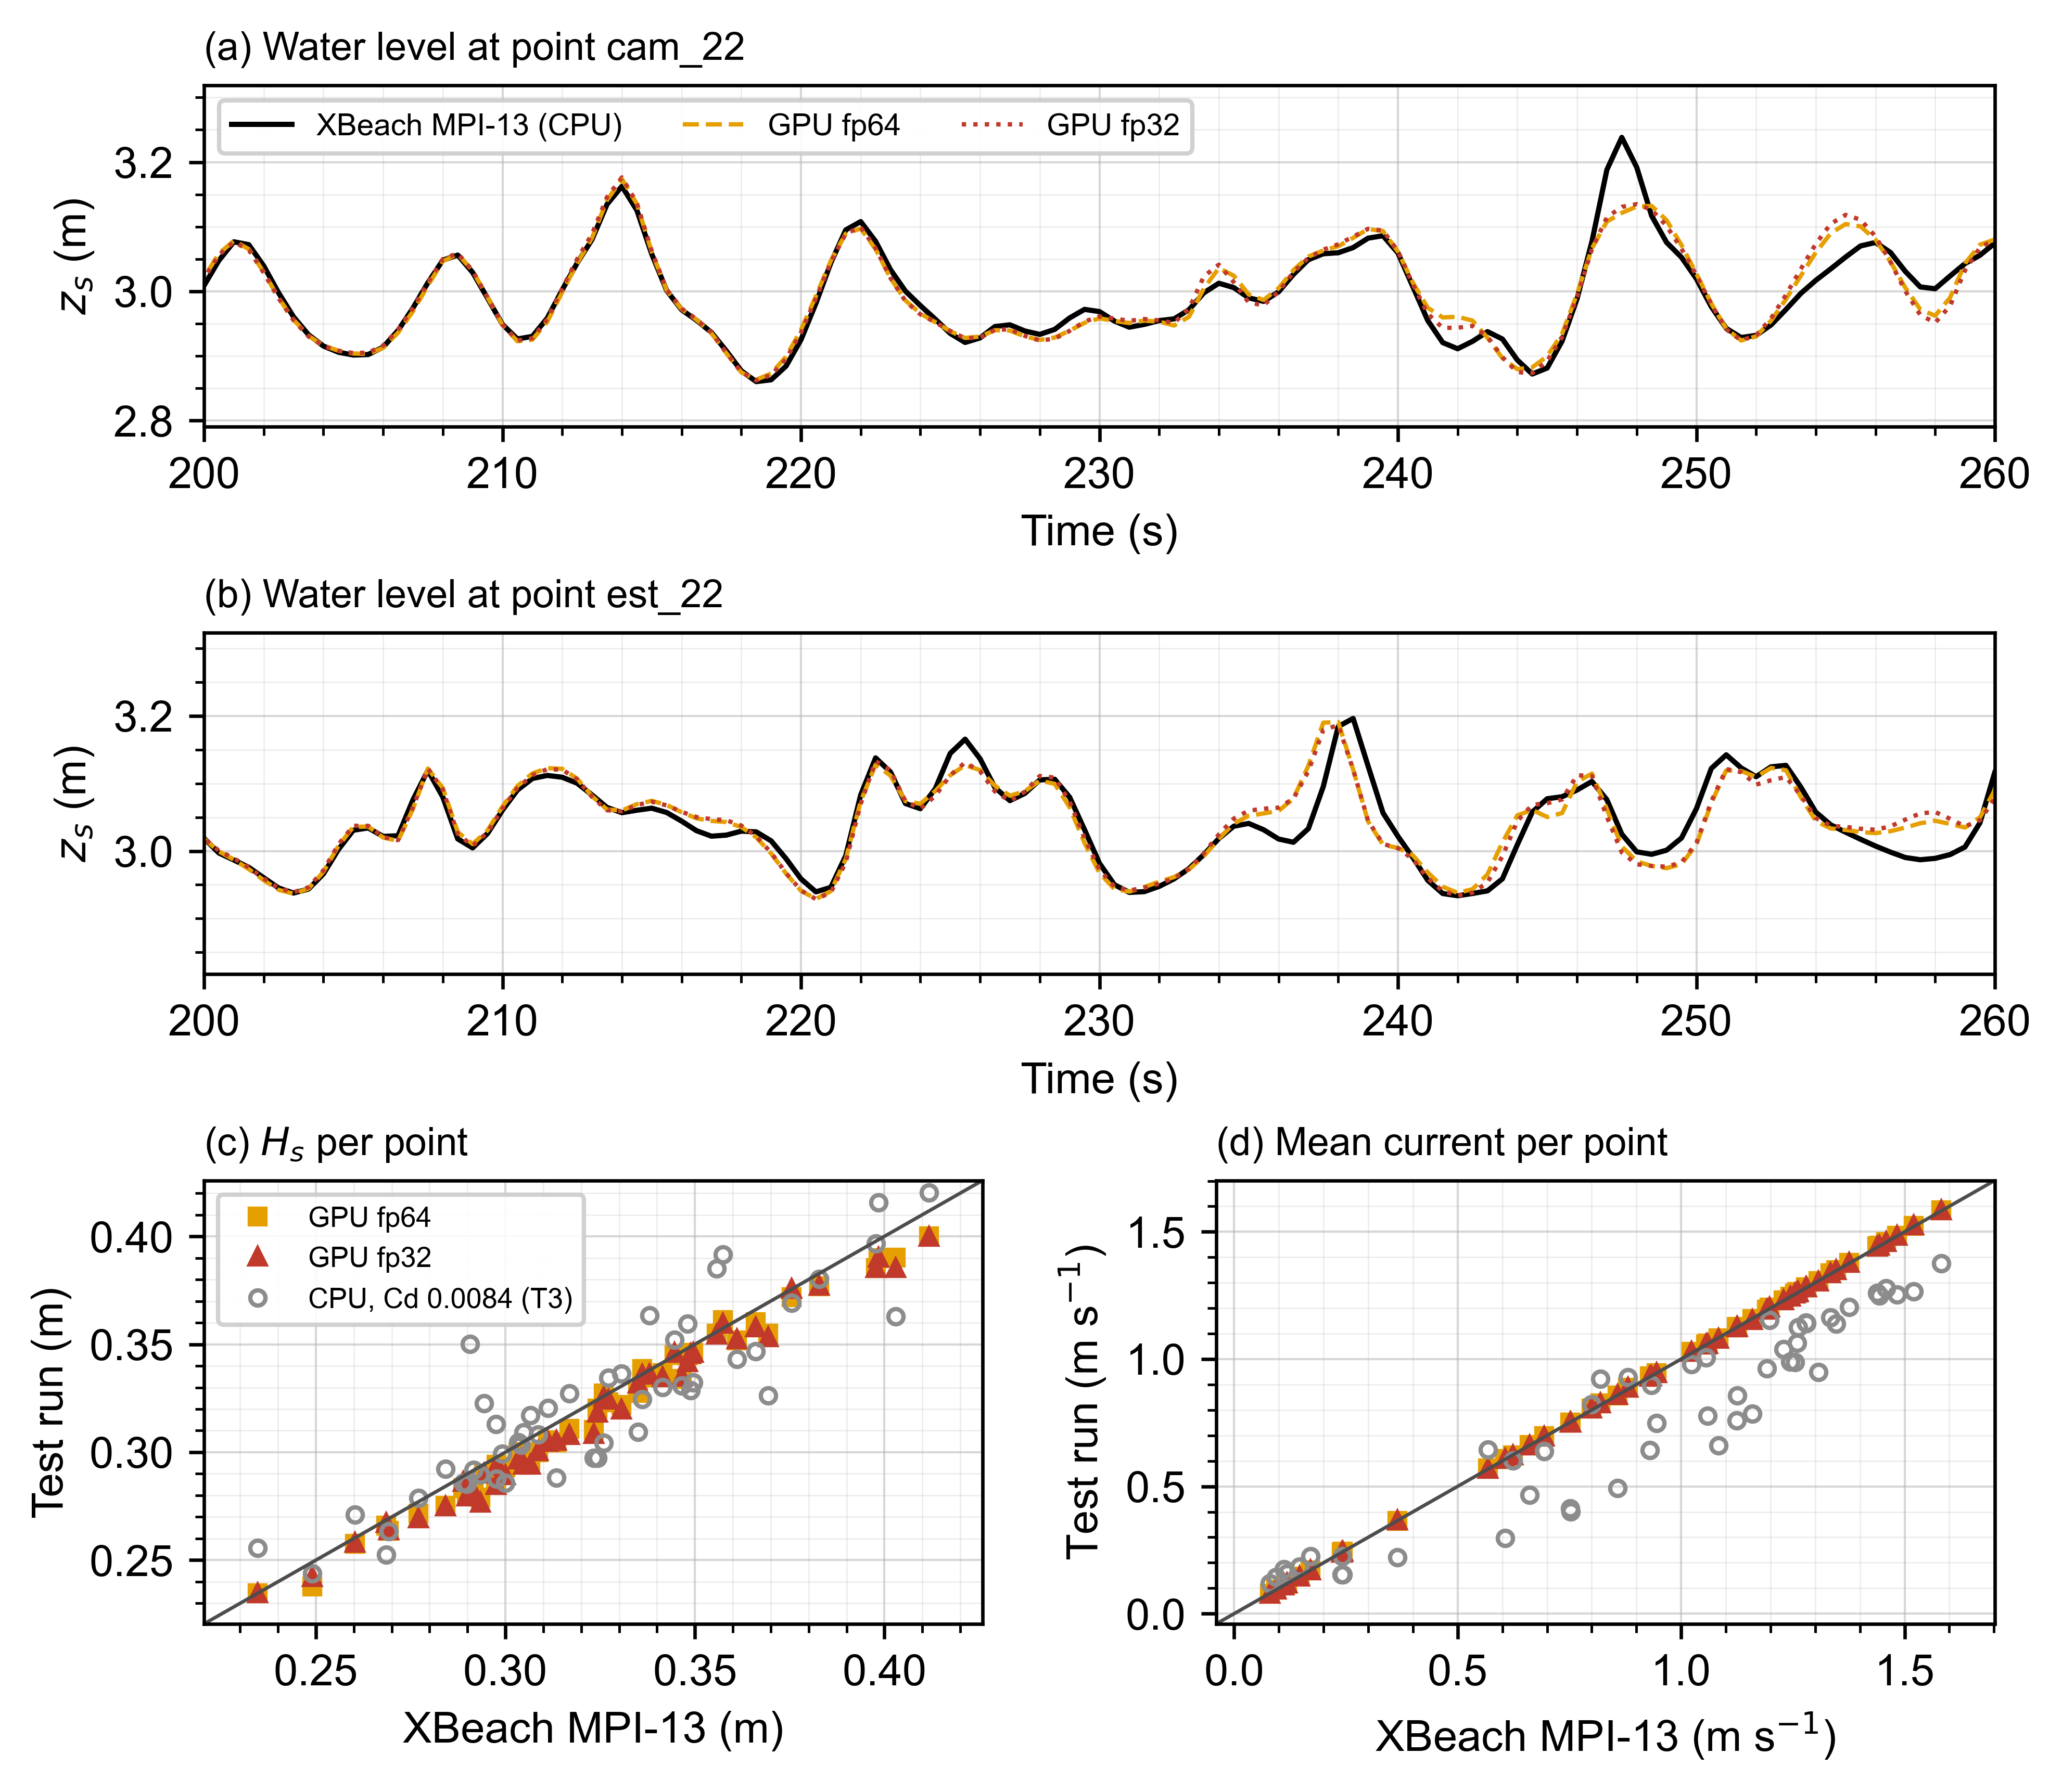
\includegraphics[width=0.82\textwidth]{estero_T0_gpu_vs_cpu.png}
\caption{Estero Island deck. (a, b) Water level at two output points; (c) $H_s$ and (d) mean current at
the 50 points: GPU against XBeach MPI-13, with a CPU wind-drag sensitivity run for scale.}\label{fig:estero}
\end{figure}

%=====================================================================================================
\section{Performance}

Table~\ref{tab:perf} lists the wall time per cell and time step on an RTX 2000 Ada (16\,GB) and an
i9-14900K (8 performance and 16 efficiency cores). The deck is the rip-channel beach, stretched
alongshore. Figure~\ref{fig:bench} shows the same benchmark.

\begin{table}[h]\centering\small
\caption{Cost per cell and time step (s).}\label{tab:perf}
\begin{tabular}{lcccc}
\toprule
Cells & XBeach MPI, best rank count & GPU fp64 & GPU fp32 & Speed-up fp64 / fp32 \\
\midrule
0.16\,M & 8.8e-8 (24 ranks) & 4.6e-8 & 2.1e-8 & 1.9 / 4.2 \\
0.63\,M & 1.0e-7 (32 ranks) & 4.6e-8 & 1.9e-8 & 2.2 / 5.5 \\
2.5\,M & 1.35e-7 (32 ranks) & 4.4e-8 & 1.9e-8 & 3.1 / 7.1 \\
8.7\,M & 1.39e-7 (24 ranks) & 4.3e-8 & 1.8e-8 & 3.2 / 7.7 \\
\bottomrule
\end{tabular}
\end{table}

\begin{figure}[h]\centering
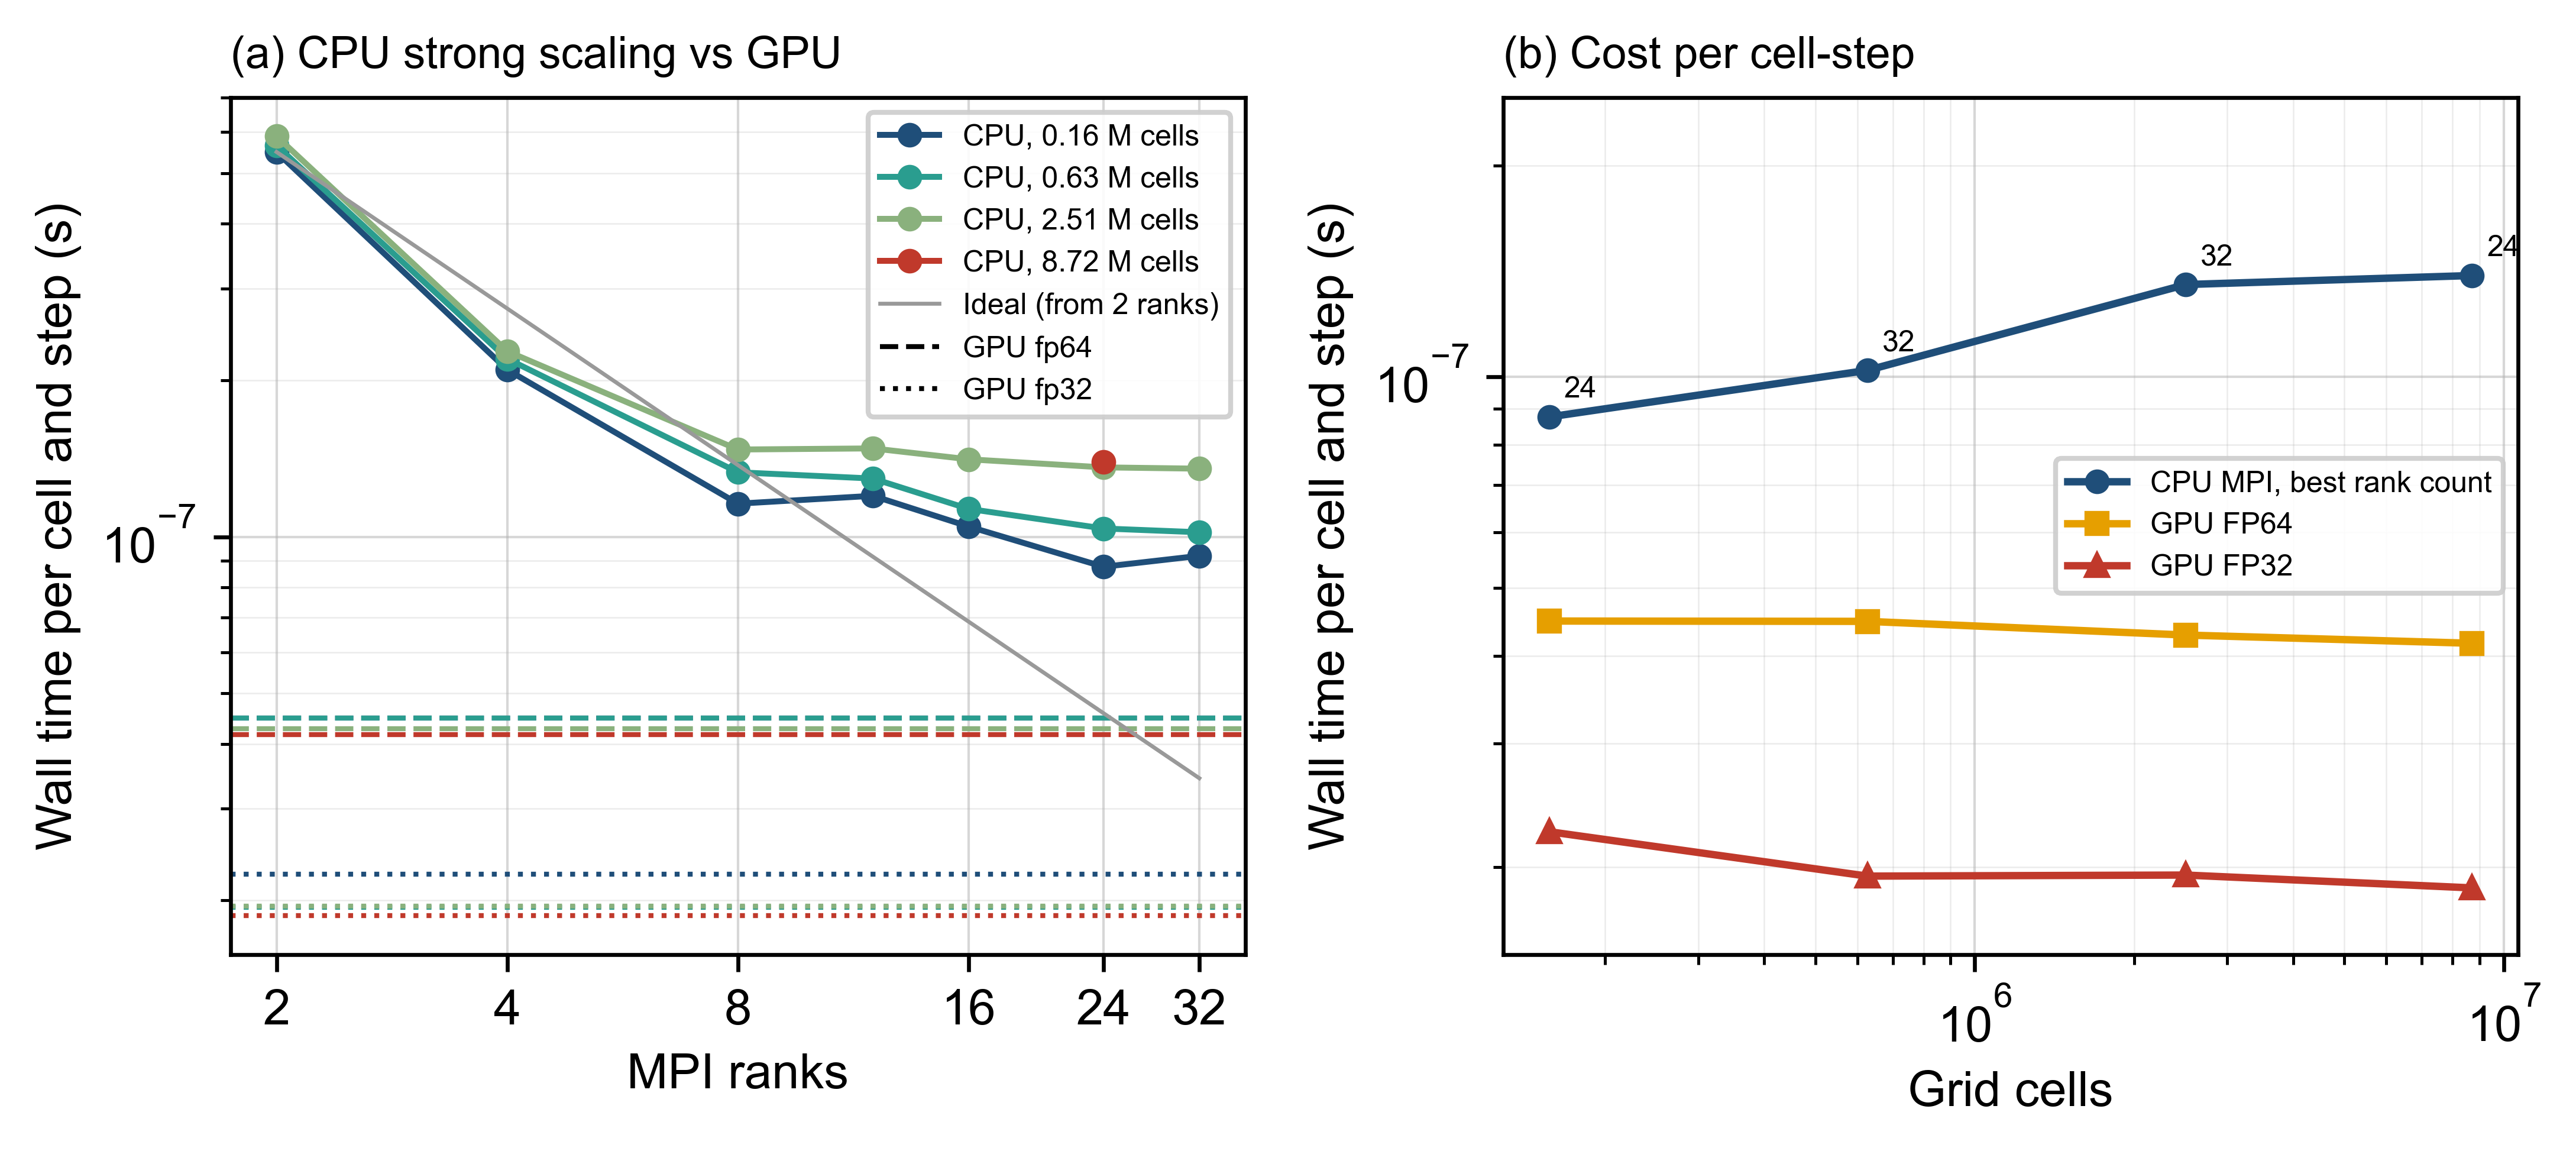
\includegraphics[width=0.9\textwidth]{benchmark_cpu_mpi_vs_gpu.png}
\caption{(a) XBeach MPI strong scaling on one workstation (lines) against the GPU (horizontal: dashed
fp64, dotted fp32); (b) cost per cell and step against grid size.}\label{fig:bench}
\end{figure}

The scaling has three features worth knowing.
\begin{itemize}
\item The CPU stops gaining beyond about 8 ranks, because all cores share the same memory bandwidth.
\item The GPU cost per cell is flat from 0.16 to 8.7 million cells.
\item The pressure solve takes about half of the GPU time.
\end{itemize}
On the Estero Island deck the 300\,s time loop took 121\,min with XBeach on 13 ranks, against 29.3\,min
(fp64) and 12.8\,min (fp32) on the GPU. A data-centre GPU (A100, H100) is expected to be another 8 to 15
times faster in double precision, but this has not been measured yet.

To reproduce the benchmark:
\begin{lstlisting}[language=bash]
SIZES="600 2400 9600" RANKS="2 4 8 16" bash tools/benchmark.sh bench
python tools/plot_benchmark.py bench/benchmark.csv
\end{lstlisting}

%=====================================================================================================
\section{Numerical notes}\label{sec:numerics}

\begin{itemize}
\item \textbf{Results do not depend on the decomposition.} The GPU domain is a single block, so results
do not change with core count. XBeach MPI results do: between 2 and 4 ranks, mean currents differ by
about 3\,\% in the tests above.
\item \textbf{One cause of the XBeach drift.} XBeach MPI exchanges \code{uu, vv} after the momentum
equation, the predictor and the second-order advection. It does not exchange them after the pressure
correction, so at each subdomain seam the continuity equation uses an uncorrected halo velocity. The
Estero hotstart files show this: their halo rows of \code{vv} differ from the rows they copy by up to
4.6\,cm/s, while \code{zs} matches exactly.
\item \textbf{Run-to-run reproducibility.} Two runs of xbnh-gpu on the same GPU agree to about
$10^{-14}$\,m, not bit for bit, because the dot products of the solver are summed with atomic
operations.
\item \textbf{Unstable corner with Neumann laterals.} With Neumann laterals and an oblique vector
boundary, the corner where the offshore and lateral boundaries meet can become unstable in both codes.
After that, the runs separate. Use cyclic laterals for oblique seas.
\end{itemize}

%=====================================================================================================
\section{Troubleshooting}

\begin{description}[style=nextline]
\item[\code{nvidia-smi} not found, or ``CUDA driver version is insufficient'']
Install or update the NVIDIA driver (525.60 or newer). On WSL2, update the Windows driver; do not install
a Linux driver inside WSL.
\item[\code{nvcc fatal: Unsupported gpu architecture 'compute\_native'}]
No GPU is visible during the build (for example on a login node). Build with \code{make ARCH=sm\_XY}
from the table in section 3.
\item[``CUDA error out of memory'']
The grid is too large for the card. Use \code{xbnh\_gpu\_sp} (about half the memory) or a larger GPU.
\item[``xbnh\_gpu: ... not supported'']
The deck uses an option outside the supported list; the message names it.
\item[``time step collapsed'']
The solution became unstable and the time step went to zero; XBeach stops in the same way. Check the
deck in XBeach first.
\item[XBeach stops with ``Missing comma between descriptors'']
This is an unpatched XBeach with output points. Use the build from \code{xbeach/build\_xbeach.sh}.
\end{description}

%=====================================================================================================
\section{License and citation}

XBeach is developed by Deltares, UNESCO-IHE and Delft University of Technology and distributed under the
GNU Lesser General Public License. xbnh-gpu translates XBeach routines to CUDA and is distributed under the
same license (LGPL-3.0). Please cite the XBeach model \cite{roelvink2009} and its non-hydrostatic breaking
formulation \cite{smit2013} when using xbnh-gpu.

\begin{thebibliography}{9}
\bibitem{roelvink2009} Roelvink, D., Reniers, A., van Dongeren, A., van Thiel de Vries, J., McCall, R.,
Lescinski, J. (2009). Modelling storm impacts on beaches, dunes and barrier islands. \textit{Coastal
Engineering}, 56(11--12), 1133--1152. doi:10.1016/j.coastaleng.2009.08.006
\bibitem{smit2013} Smit, P., Zijlema, M., Stelling, G. (2013). Depth-induced wave breaking in a
non-hydrostatic, near-shore wave model. \textit{Coastal Engineering}, 76, 1--16.
doi:10.1016/j.coastaleng.2013.01.008
\end{thebibliography}

\end{document}
